%-----------------------------------------------------------------------
% Subsection: Motivating example
%-----------------------------------------------------------------------
\section{Motivating Example}
\label{sec:problem}

In order to customize specific products, by selecting a valid feature
configuration, variation points must be represented in the product line
artifacts. Several notations for representing variation points in use case
scenarios have been proposed, such as Product Line Use Cases
(PLUC)~\cite{Bertolino:2003aa} and Product Line Use Case Modeling for Systems
and Software Engineering (PLUSS)~\cite{Eriksson:2005aa}. However, in spite of
the benefits of variability representation, existing approaches do not present
a clear separation between variability management and scenario specifications. In this
section we illustrate the resulting problems using the \emph{eShop Product
Line}~\cite{Pohl:eshop} as a motivating example.

The primary use cases of the \emph{eShop Product Line} (EPL) allow the user to
\emph{Register as a Customer}, \emph{Search for Products}, and \emph{Buy
Products}.  Five variant features are described in the original specification,
corresponding to a product family composed of 72 valid
configurations~\cite{Pohl:eshop}. In this paper we consider additional features
and use cases, such as \emph{Update User Preferences}, which updates the user's
preferences based on her historical data of searches and purchases.

Figure~\ref{fig:eshop-fm} presents part of the
EPL feature model~\cite{Gheyi:2006aa,Czarnecki:2000aa}, which represents the
common and variable features of our example. Here we represent it by a tree like
notation where relationships between a parent feature and its children are
categorized as \emph{Optional} (features that might not be selected in a specific product), \emph{Mandatory} (feature that must be selected, if the parent
is also selected), \emph{Or} (one or more subfeatures might be selected), and
\emph{Alternative} (exactly one subfeature must be selected for each product).
Besides these relationships, feature models allow the specification of
constraints among features. For instance, the constraint ($Shopping\ Cart\
\Leftrightarrow\ Bonus$) states that the feature Shopping Cart is selected iff
the feature Bonus is also selected.

 \begin{figure}[th]
 \begin{center}
  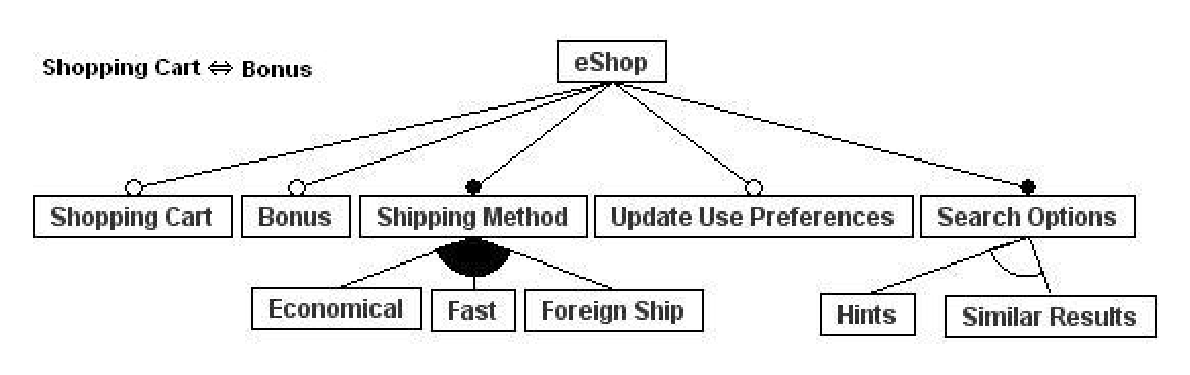
\includegraphics[scale=0.45]{img/eShop-FM.eps}
   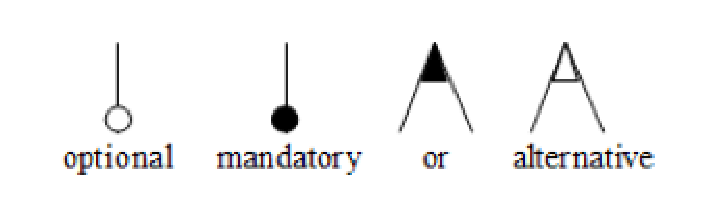
\includegraphics[scale=0.40]{img/fm-notation.eps}
  \caption{eShop feature model.}
  \label{fig:eshop-fm}
  \end{center}
\end{figure}


%Other approaches are based on use case extensions~\cite{jacobson-reuse-book}, not explored here since they
%require that one use case extension must be defined for each variant. This can result in a huge
%number of use cases that is not suitable for managing activities.


Figure~\ref{fig:pluss-01} depicts the \emph{Buy Product} scenarios written in
the PLUSS notation. Notice that a single artifact is used to represent all valid
configurations related to this scenario, mixing common behavior, variant
behavior, and configuration information (feature selection inside square
brackets). For example, steps 1(a) and 1(b) are never performed together. They
are alternative steps: Step 1(a) will be present only if the \emph{Shopping
Cart} feature is selected, otherwise Step 1(b) will be present. In a similar
way, we have to choose between options (a) and (b) for Step 2 (depending whether
the \emph{Bonus} feature is selected or not). Finally, Step 6 is optional and
would be present only if the feature \emph{Update User Preference} was selected.

As a consequence, since all possible variants are described in the same
artifact, PLUSS approach presents difficulties for understanding the behavior
of specific products.
Moreover, this tangling between \emph{common} and
\emph{variant} behavior results in maintainability issues: introducing a new product variant
requires changes in several points of existing scenarios. For example, including a
\emph{B2B Integration} feature, which allows the integration between partners in
order to share their warehouses, changes the specification of the \emph{Buy
Product} scenario, enabling the search for product availability in remote
warehouses (a new variant for Step 1) and updating a remote warehouse when the
user confirms the purchase (a new variant for Step 5). Moreover, the inclusion of
this new optional feature also changes the specification of the \emph{Search for
Products} scenario (the search might also be remote). The effort
needed to understand and evolve a product line increases, since the
specification of certain features is scattered through several scenarios,
and each scenario describes several configurations.

% In the PLUSS notation, this kind of relationship between
% features and scenarios is scattered throughout different scenarios.


\begin{figure}[h]
\begin{center}
\begin{scriptsize}
  \texttt{
  \begin{tabular}{||p{0.2in}||p{1.3in}||p{1.3in}||}
   \hline
	Id    & User Action & System Response \\ \hline \hline
       1(a) &Select the checkout option. \mbox{[ShoppingCart]}& Present the
       items in the shopping cart and the amount to be paid. The user can remove
       items from shopping cart. \\  \hline 1(b) & Select the buy product
       option. \mbox{[not ShoppingCart]} & Present the selected product. The
       user can change the quantity of items that he wants to buy. Calculate
       and show the amount to be paid. \\  \hline 2(a) & Select the confirm option. [Bonus]& Request bonus and payment information. \\  \hline 2(b) & Select the confirm option. [not Bonus]& Request payment
       information. \\  \hline 3     & Fill in the requested information and select the proceed option. & Request the shipping method and address.\\  \hline 4     & Select the \$ShippingMethod\$, fill in the destination address and select the proceed option. & Calculate the shipping costs. \\  \hline
       5     & Confirm the purchase. & Execute the order and send a request to the Delivery System in order to dispatch the products. \\  \hline
       (6)     & Select the close session option. \mbox{[Update User
       Preferences]} & Register the user preferences.\\  \hline
  \end{tabular}
  }
\end{scriptsize}
\caption{Buy Products scenarios using the PLUSS.}
\label{fig:pluss-01}
\end{center}
\end{figure}



% Section~\ref{sec:evaluation} presents a quantitative study regarded to the PLUSS'
% maintanability issues.

% For example, including a \emph{B2B Integration}
% feature, which allows the integration between partners in order to share their warehouses, might change the specification of the \emph{Buy
% Product} scenario, enabling the search for product availability in remote
% warehouses (a new variant for Step 1) and updating a remote warehouse when the
% user confirms the purchase (a new variant for Step 5). Moreover, the inclusion of
% this new optional feature also changes the specification of the \emph{Search for
% Products} scenario (the search might also be remote). In summary, since the
% behavior of certain features may be spread among several specifications and each
% specification might describe several variants, the effort needed to understand
% and evolve the product line might increase.


Differently, PLUC introduces special tags for representing variation points in
use case scenarios. For example, the VP1 tag in Figure~\ref{fig:pluc-01}, which also
describes the \emph{Buy Products} scenario, denotes a variation point that might
assume the values ``\emph{checkout}'' or ``\emph{buy product}'', depending on
which product is being configured. For each \emph{alternative} or
\emph{optional} step, one tag must be defined. The actual value of each tag is specified in the
\emph{Variation Points} section of a scenario specification.

\begin{figure}[h]
\begin{center}
\begin{scriptsize}
  \texttt{
  \begin{tabular}{{||p{0.05in}p{3in}||}}
  \hline
  & {\bf Buy Products Scenario} \\
  & {\bf Main Flow} \\
  01 & Select [VP1] option \\
  02 & [VP2] \\
  03 & Select the confirm option \\
  04 & [VP3] \\
  05 & Fill in the requested information and select the proceed option \\
  06 & Request the shipping method and address \\
  07 & Select the [VP4] shipping method, fill in the destination address and select the proceed option \\
  08 & Calculate the shipping costs. \\
  09 & Confirm the purchase. \\
  10 & Execute the order and sends a request to the Delivery System in order to dispatch the products \\
  11 & Select the close section option. \\
  12 & \{[VP5] Register the user preferences.\} \\  & \\
  & {\bf Products definition: } \\ & VP0 = (P1, P2) \\ & \\
  & {\bf Variation points: } \\
  &  VP1 =  if (VP0 == P1) then (checkout) \\ & \hspace{0.25in} else (buy product) \\
  & VP2 =  if (VP0 == P1) \\ & \hspace{0.25in}  then (Presents the items in the shopping cart...) \\ & \hspace{0.25in} else (Present the selected product. The user...) \\
  & VP3 =  if (VP0 == P1) \\ & \hspace{0.25in} then ( Requests bonus and payment information.) \\ & \hspace{0.25in} else (Requests payment information.) \\
  & VP4 =  (Economic, Fast) \\
  & VP5 requires (VP0 == P1) \\ \hline
   \end{tabular}
  }
\end{scriptsize}
\caption{Buy Products scenarios using the PLUC.}
\label{fig:pluc-01}
\end{center}
\end{figure}

Another kind of tangling occurs in this case. the specification of common and
variant behavior are separate, but both are tangled to the variation points.
Additionally, SPL members are also described using the same tag notation (see the
\emph{Products Definition} section in Figure~\ref{fig:pluc-01}). There is no
explicit relationship between product configurations and feature models. In the
example, two products (P1 and P2) are defined. The first product is configured by
an implicit selection of the \emph{Shopping Cart}, \emph{Bonus}, and \emph{Update
User Preferences} features; in contrast to the second product that is not
configured with these features.


As the values of alternative and optional variation points are computed based on
the defined products, instead of specific features, the inclusion of a new member
in the product line might require a deep review of the \emph{Variation Points}
section in many scenarios. Moreover, since the variation points and the product
definitions are spread among several scenario specifications, it is hard and time
consuming to keep consistent the relationships between them. Finally, the same
definitions (product configuration and variation points) are often useful to manage variabilities in other artifacts, such as design and source code. As a consequence, this approach
requires the replication of such definitions in different SPL views.


In conclusion, both PLUSS and PLUC do not present a clear separation between
variability assets and scenario specifications, which compromises the
evolution of a SPL. Besides that, both approaches rely on simple
variability techniques: filtering optional steps in scenarios, or syntactic
changes of tag values based on product definition. In this sense, according to the terminology
presented in~\cite{Kastner:2008aa}, they can be classified as \emph{annotated
techniques}, which are not suitable for modularizing the crosscutting nature of certain
features, have poor legibility, and lead to lower
maintainability~\cite{Alves:2006aa,Kastner:2008aa}.

% For this reason, Pohl et al. argued that the
% variability management concern should be separated from the other SPL
% assets~\cite{Pohl:2005aa}. However, besides the use of independent models for
% representing the variability concern, it is also necessary concrete descriptions
% of the composition processes used to generate specific products.


% this case, in order to support the automatic derivation of product specific
% artifacts, it is necessary not only to have a more precise definition of each
% language used to describe product line artifacts and the variability management
% concern, but also to formalize the weaving processes used to combine them.
%
% The
% PLUSS and PLUC approaches fail in this direction, since Eriksson et al. defines
% the metamodel of PLUSS notation~\cite{eriksson-splc-2005}, but do not describe
% which languages and processes are used for relating use case scenarios to feature
% models. Likewise, although Fantechi et al. describe the formal semantics of
% PLUC~\cite{fantechi-splc-2004}, this approach does not separate variability
% management from use case scenarios.

% Next section describes our approach, named as Scenario Variability as
% Crosscutting Mechanisms (SVCM), which deals with scenario variability
% management by means of the composition of different artifacts. A key
% characteristic found in SVCM is that each involved artifact has a clear and
% specific contribution to the SPL engineering.

% Although in this paper we are focus on use
% case scenarios, the idea of separating product line artifacts from variability
% management (using feature models, product configurations, and configuration
% knowledge) is also applied to other SPL views. 